\documentclass[10pt,twocolumn,letterpaper]{article}

\usepackage{cvpr}
\usepackage{times}
\usepackage{epsfig}
\usepackage{graphicx}
\usepackage{amsmath}
\usepackage{amssymb}
\usepackage{algpseudocode}% http://ctan.org/pkg/algorithmicx
\usepackage{algorithm}% http://ctan.org/pkg/algorithm
\usepackage{subfig} %for subfigure environment
\usepackage{multirow}
\usepackage{array}
\usepackage{url}
%\usepackage{bbm}


\usepackage[normalem]{ulem}

\newcommand{\argmax}{\operatornamewithlimits{argmax}}
\newcommand{\argmin}{\operatornamewithlimits{argmin}}
\newcommand{\eqdef}{\overset{\mathrm{def}}{=\joinrel=}}


% Include other packages here, before hyperref.

% If you comment hyperref and then uncomment it, you should delete
% egpaper.aux before re-running latex.  (Or just hit 'q' on the first latex
% run, let it finish, and you should be clear).
\usepackage[pagebackref=true,breaklinks=true,letterpaper=true,colorlinks,bookmarks=false]{hyperref}

\cvprfinalcopy % *** Uncomment this line for the final submission

\def\cvprPaperID{118} % *** Enter the CVPR Paper ID here
\def\httilde{\mbox{\tt\raisebox{-.5ex}{\symbol{126}}}}

% Pages are numbered in submission mode, and unnumbered in camera-ready
\ifcvprfinal\pagestyle{empty}\fi
\begin{document}

%%%%%%%%% TITLE
\title{Interactive Action Recognition using Relative Geometry Between Body Parts Across Multiple People}

\author{Swami Sankaranarayanan, Kota Hara, Yiannis Aloimonos\\
Center for Automation Research, University of Maryland, College Park, MD 20742\\
{\tt\small \{swamiviv,kotahara\}@umiacs.umd.edu yiannis@cs.umd.edu}
% For a paper whose authors are all at the same institution,
% omit the following lines up until the closing ``}''.
% Additional authors and addresses can be added with ``\and'',
% just like the second author.
% To save space, use either the email address or home page, not both
}


\maketitle
%\thispagestyle{empty}

%%%%%%%%% ABSTRACT
\begin{abstract}
In this work, we propose
   
\end{abstract}

%%%%%%%%% BODY TEXT
\section{Introduction}
Human action recognition has been a major problem in computer vision community for many years. There are many applications of the human action recognition such as surveillance, health-care and human computer interaction. Most of the previous works focus on action recognition of a single person. The action classes considered in this scenario is limited to a simple action such as walking, running and jumping. 

On the other hand, there are several works which deal with action classes involved with multiple people. These action classes are more complex to recognize than the single-person actions due to the complexity of the actions. The actions are defined not only by the motion of one person but also their interactive motions. We call these multiple-people actions as interactive actions.

The examples of interactive actions we consider in this work are exchanging objects and greetings between two people. For exchanging objects, we consider different types of the objects such as cards, a ball and a chair. Depending on the object being exchanged, their interactive movement come out in a different form. For greetings, we consider interactive actions such as shaking hands and bowing. Our goal is to recognize these different types of interactive actions from the 3d skeleton information.


Action recognition from the body skeleton information has been actively studied due to the advance of motion capture systems such as Kinect. Typically the skeleton information is given in the form of 3d locations of a set of body joints. Many action recognition systems directly use these information as the input or convert the location information into a set of joint angles and then use them as the input. The focus of most of the previous research has been on the recognition part. 

\cite{Vemulapalli2013} proposed a new skeleton representation based on relative geometry across body parts and achieve the state of the art results on several standard single-person action recognition datasets. They compute the translation and rotation between each pair of body parts and map it to the tangent space to obtain a feature vector. The benefit of their approach compared to the previously adopted skeleton representation is that their representation can directly capture the relationship between body parts that are not directly connected each other. Thus, it is more capable of recognizing actions in which the relationship between non-connected body parts, such as left arm and right arm, is more important.

In this work, we extend \cite{Vemulapalli2013} to classify actions performed by two people. In our skeleton representation, in addition to the relative geometry across body parts within one person, we also consider relative geometry between body parts across two people. We believe that this representation enables us to capture two people's interaction well. For instance, our representation can captures the geometric relationship between a left arm of a person A and a right arm of a person B, which might be helpful to recognize the 'shaking hands' actions.

For the recognition part, we develop an algorithm to automatically detect frames where actions are taking place. For each sequence, we computer the proposed skeleton features at each frame in the detected periods of the frames. Then we sample a fixed number of features with the constant interval by a simple interpolation method. This way we obtain the same number of features from each detected period. We concatenate these features and use it as an input to multiclass classifiers.

The paper is organized as follows. In section 2, we show some related work. Section 3 explains our action localization method. Then we describe, in section 4, the proposed skeleton representation at each frame. Section 5 presents the interpolation method to obtain a final feature vector as well as the classification methods we propose. The experimental results are shown in section 6, followed by the conclusion in section 7.


\section{Related Work}

\section{Action Localization}
The action sequences that are collected from the Kinect consists of several irrelevant frames which does not contain the action that we are looking for. Thus, given a video sequence it becomes important to approximately localize the action. This is a mandatory pre-processing step to extract realiable features that completely describe the action that  we are interested in. We alos assume throughout this work that there is only one continuous action that takes place throughout a given video sequence. In this section, we decribe a heuristic way to localize the action in a given video. A given video sequence consists of the following parts:
\begin{equation}
<Init. Action - Main Action - Finish>
\end{equation}
The heuristic described here tries to acquire the frames corresponding to the Main Action  in an automated way. We perform the localization in two steps:
\begin{itemize}
\item Computing the action center frames
\item Computing the start and end frames
\end{itemize}

The action center frame is computed as the frame where the distance between the interacting persons is the least. If there are multiple frames with the same distance value (this could occur since some interactions can last for a few frames), the action center frame is assigned as the minimum of those frames.

The start(end) of any interaction in the video could be implied by a constant decrease(increase) in distance between two persons. Thus, we compute the distance between the persons at each frame and identify when the rate of change of distance goes above(start) or below (end) a given threshold $\delta$, which is a user input parameter. 


As can be observed, this method does not yield us exact localization but an approximate one. In the subsequent section, we take care of this by imposing temporal smoothness on the features that we extract from each frame. 
\section{Skeleton Representation}


The output from the Kinect sensor is 3d positions of 20 body joints for each person defined in the global coordinate. We define our skeleton representation for the first person as $S^{(1)}=(V^{(1)},E^{(1)})$, where $V^{(1)}=\{v_{1}^{(1)},v_{2}^{(1)},\dots,v_{N}^{(1)}\}, N=20$ denotes the set of joints and $E^{(1)}=\{e_{1}^{(1)},e_{2}^{(1)},\dots,e_{M}^{(1)}\}, M=19$ denotes the set of body parts ( See Fig.\ref{fig:skeleton}). Let $e_{m1}^{(1)},e_{m2}^{(1)} \in \mathcal{R}^3$ represents the starting and ending points of the body part $e_{m}^{(1)}$. Similarly we have $S^{(2)}=(V^{(2)},E^{(2)})$ for the second person.

First, we define the person specific local coordinate at the first person's shoulder center computed as $(v_5 + v_6)/2$ such that the x coordinate is aligned with the person's body orientation. Then we update both $S^{(1)}=(V^{(1)},E^{(1)})$ and $S^{(2)}=(V^{(2)},E^{(2)})$ using this new coordinates. This process makes our representation invariant to the global translation and orientation. 

Next we consider a set of body parts, $E=\{E^{(1)},E^{(2)}\}$, and for each pair of body parts $e_m$ and $e_n$, in $E$, we describe their relative geometry by the translation and rotation. The translation is computed as $T_{m,n}=e_{m1}-e_{n1}$. For the rotation, we compute the rotation axis $r$ and the rotation angle $\theta$ between two vectors $e_{n2}-e_{n1}$ and $e_{m2}-e_{m1}$. From them we compute a quaternion $q_{m,n} \in \mathcal{R}^4$ by $q_1=r_1 sin( \frac{\theta}{2} ), q_2=r_2 sin( \frac{\theta}{2} ), q_3=r_3 sin( \frac{\theta}{2}), q_4=cin( \frac{\theta}{2})$.

Thus, each pair of parts can be represented as 7 dimensional vector. Since there are $\binom{38}{2}$ such pairs, we have $\binom{38}{2} \times 7 = 4921$ dimensional vector. We do the same step by using the second person's local coordinate and concatenate two vectors to obtain the final 9842-d feature vector representing two people configurations at a current frame.

\begin{figure}[htb]
\begin{center}
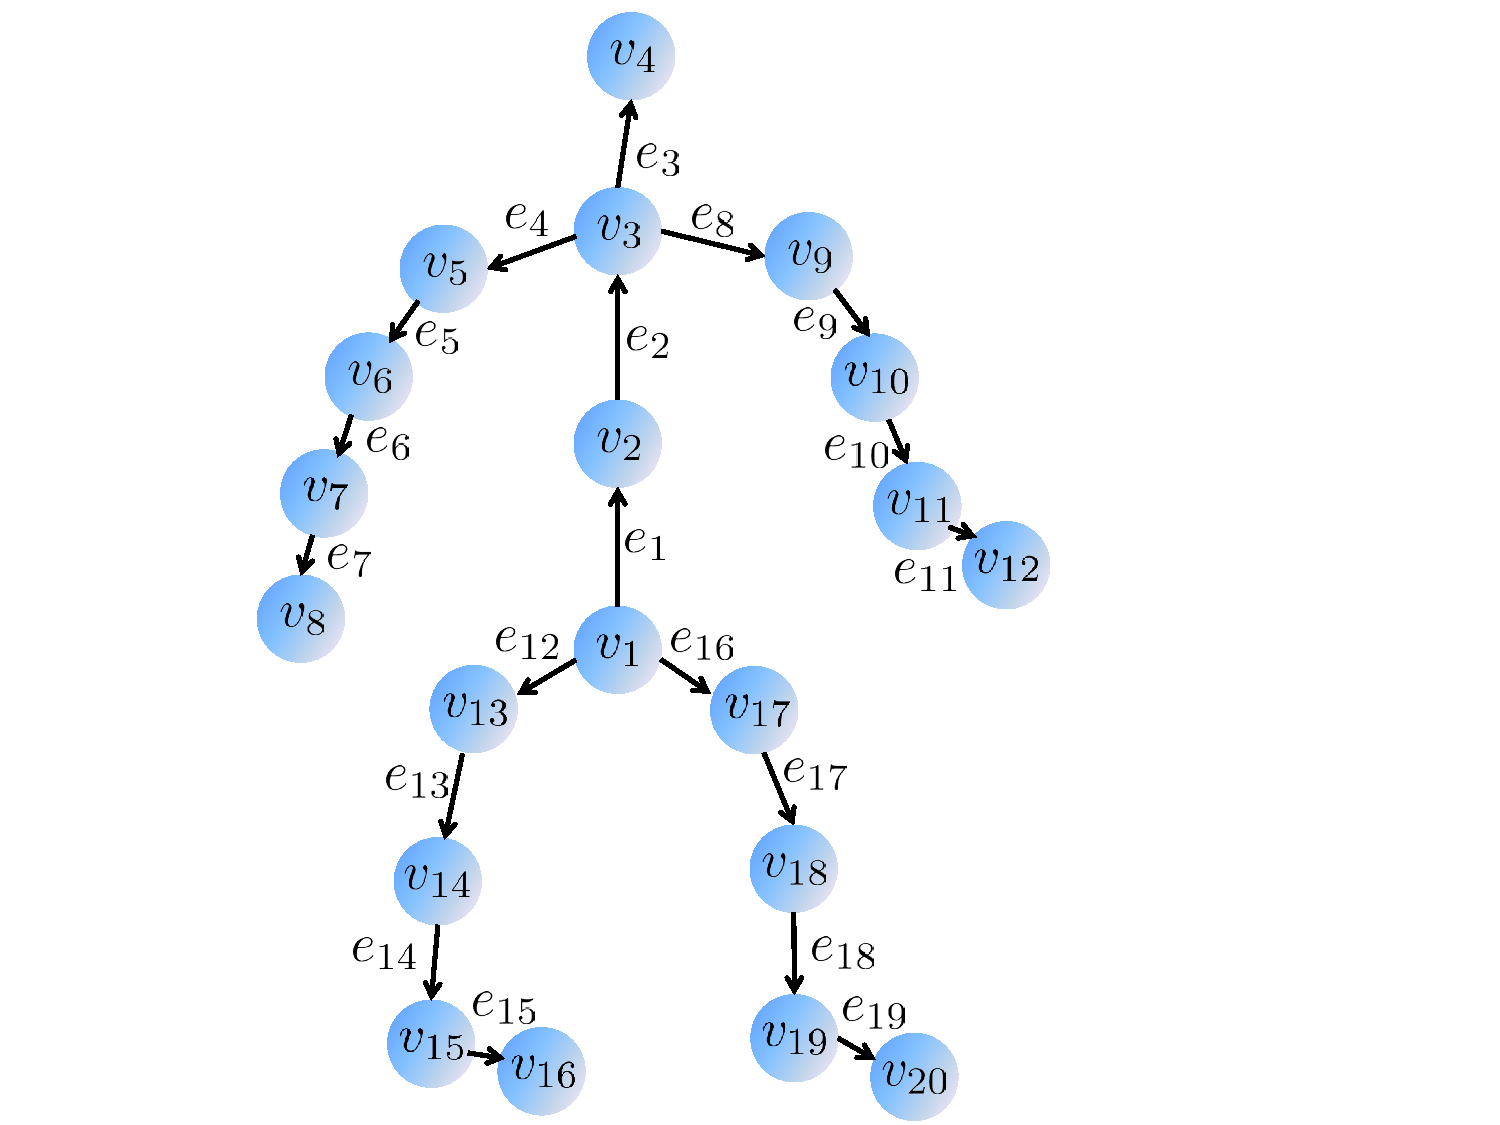
\includegraphics[width=2.3in]{skeleton.pdf}
\caption{An illustration of the skeleton. \label{fig:skeleton}}
\end{center}
\end{figure}

To extract features from one action sequence, we first compute our skeleton feature across frames detected by the action localization algorithm. Since the length of the detected action frames is different across sequences, we apply temporal interpolation to sample skeleton features at 30 uniformly distributed time instance. We then apply PCA to reduce the dimensionality to 1000. Finally, we concatenate all the vectors into 30000-d feature vector.

\section{Action Classification}
We propose two different methods for classifying interactive actions from the skeleton features.

\subsection{Generative Modeling}
Given an input video containing the action, generate a semantic desription of the action as it occurs in the video. To describe an action would mean to generate a dictionary based representation for the action. A suitable middle ground between a complete linguistic action definition and a machine-derivable description, we borrow the action vocabulary decribed in \cite{SUHA}. Accordingly, a single person action in general can be described using an \textbf{operational triplet} as follows:

\begin{equation}
<Agent-Motion-Target>
\end{equation}

where $Agent$ is the person or the body part of the person which initiates the action; $Motion$ implies the movement of the $Agent$; $Target$ can be taken to be an object or another person or his body part that is involved in the interaction. Using this terminology some simple action representations can be generated as shown below:

\begin{itemize}
\item \textbf{Handshake}: $<$Arm1 - Outstretched - Arm2$>$
\item \textbf{Kicking}: $<$Leg1 - Outstretched - Leg2$>$
\end{itemize}

It should be noted that for some actions that \textit{Agent} and \textit{Target} need not necessarily be a single person or body part but can be a collection of body parts that act on each other in a causal way. To see an example of this, consider the figure \ref{Fig:act_des}

\begin{figure}[ht]
\centering

  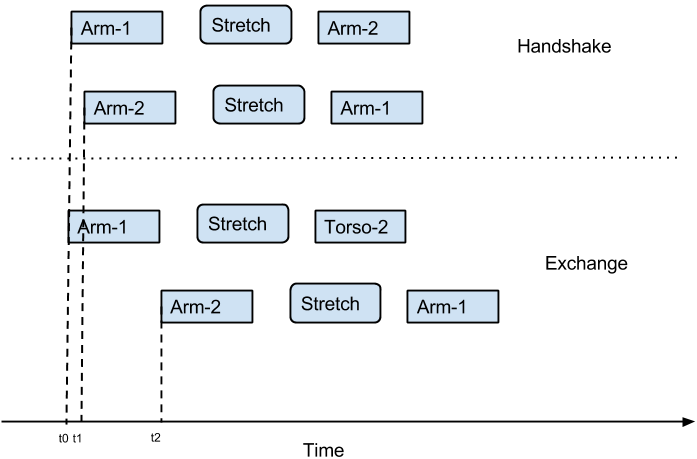
\includegraphics[scale = 0.3]{action_des.png}%
  \label{Fig:act_des}%

\end{figure}

Thus, we can see that actions that have similar semantic descriptions in terms of the operational triplet can be differentiated by means of proper temporal constraints. To look at how spatial constraints can decide the type of interaction, we incorporate that knowledge in the decision tree structure shown in figure \ref{Fig:tree}.

\begin{figure}[ht]
\centering

  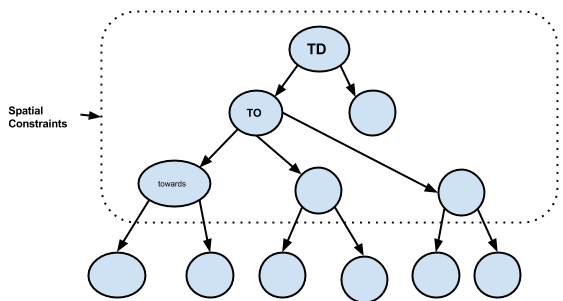
\includegraphics[scale = 0.3]{dec_tree.png}%
  \label{Fig:tree}%

\end{figure}

\subsection{Artificial Feed-forward Neural Network}
We use artificial feed-forward neural network with softmax activation function as its final layer to estimate conditional probability, $P(y_t|x_t,t=t_{ac})$ at time instance $t$, where $y_t$ is an action class label and $x_t$ is the skeleton features computed from $t-20$ to $t+20$ frames and $t_{ac}$ is the time instance of the action center frame. We manually localize the action center frame of the training sequences and train the model with 10 hidden layers.

In testing time, we apply the trained neural network in a time sliding window manner and obtain the conditional probability $P(y_t|x_t,t=t_{ac})$. We also apply our action center detector at each frame to obtain $P(t=t_{ac}|x_t)$. We then compute $P(y_t,t=t_{ac}|x_t)=P(y_t|x_t,t=t_{ac}) P(t=t_{ac}|x_t)$ at each frame. Finally, we compute $P(y)$ for each sequence by $\sum_{t=t_{s}}^{t_{e}} P(y_t,t=t_{ac}|x_t)$ where $t_{s}$ and $t_{e}$ are the time instance where there are sufficient number of frames to apply the neural network. The final prediction is done by $\argmax_{y} P(y)$.

\section{Experiments}

\subsection{Data Collection}

We create a new dataset named Maryland Interactive Action Dataset (MIAD) which consists of 10 interactive action classes captured by Kinect. The action classes we consider are summarized in Fig.\ref{fig:newactions} with their representative images. For each pair of people, we collect 2 sequences per an action class by switching their locations. Since we collect data from 6 pairs of people, there are 12 sequences per action class. We use the first X sequences as training data and the remaining sequences as testing data.

\begin{figure*}[htb]
\begin{center}
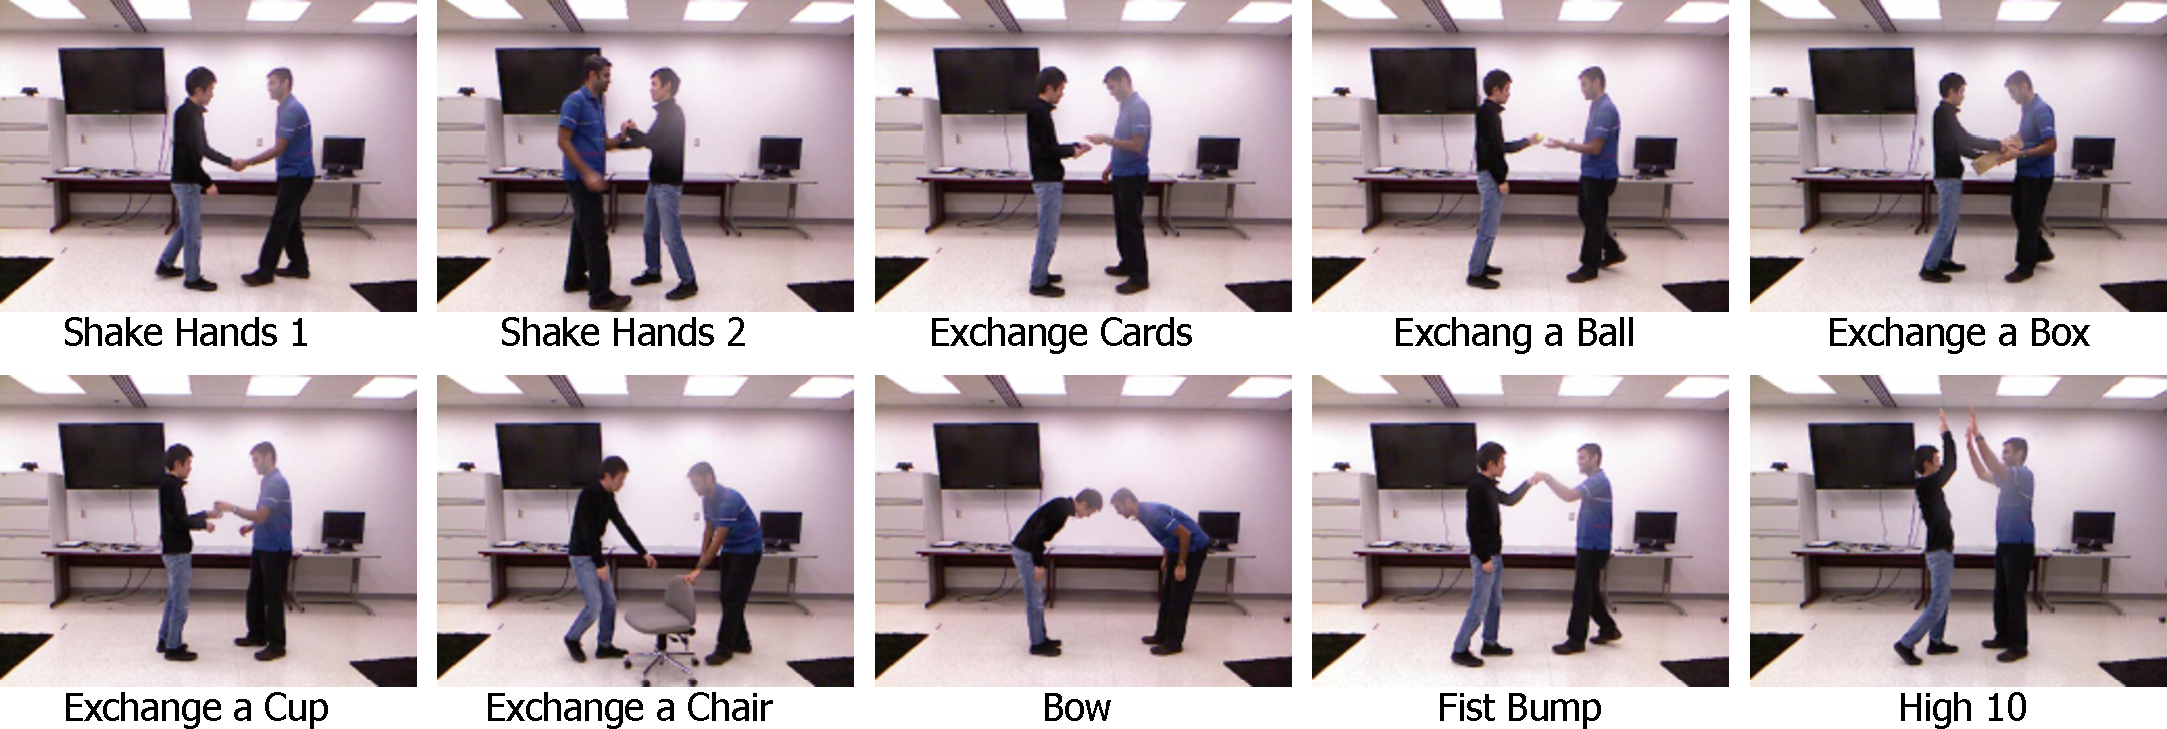
\includegraphics[width=6.8in]{newactions.pdf}
\caption{Action classes in newly collected MIAD dataset.  \label{fig:newactions}}
\end{center}
\end{figure*}

Our new data, MIAD differs from the existing two people interactive dataset such as K3HI \cite{K3HI} and SBU Kinect Interaction Dataset \cite{Yun2012}. First, our skeleton is represented by 20 joints whereas K3HI and SBU have only 15 joints. Second, the action classes we consider are more 'fine-grained'. In K3HI and SBU, there is only one action class for 'exchanging an object' class while MIAD contains 5 unique action classes for it, differentiated by the object being exchanged. Also K3HI and SBU have only one action class for the greeting action, namely, shaking hands, while MIAD includes 5 different action classes. These fine-grained actions are generally more challenging to discriminate as actions are more similar each other, necessitating more detailed representation of body movements.

%Steps for performing Interaction Recognition using Kinect:

%Step 0 : To organize the data in the above format. To do this, we extract skeleton data from the recorded OpenNI files that comes from the Kinect sensor.

%Step 1 : For each frame, we have to spatially localize each person - We are trying to figure out how to extract this information directly from the Kinect output

%Step 2 : Should perform an Object Detection routine to verify if there is any sign of Object exchange

%Step 3 : Based on how each joint moves in the video per frame, the activity trees are grown and the corresponding activity is detected. Primarily we want to differentiate between Object/Non-object Interactions and further classify the Non-Object Interactions into one of the Action classes that were given to us during Training. 

%The skeleton representation provides a convenient way to represent different actions in the form of Action trees. The terminal nodes of each action tree consists of the 20 joint positions. For each action, based on how different joint nodes combine to perform that action we can develop the corresponding action tree. 

\subsection{Action Localization Results}
Show the examples of the starting frame, center frame and the ending frame.

\subsection{Action Classification Results}
Show confusion matrix.
Give some discussion on difficult action classes.

\section{Conclusion}


\begin{thebibliography}{9}

\bibitem{Vemulapalli2013}
  Raviteja  Vemulapalli,
  Felipe Arrate,
  Rama Chellappa,
  \emph{Human Action Recognition by Representing 3D Skeletons as Points in a Lie Group}.
  CVPR,
  2014.

\bibitem{SUHA} Semantic-level Understanding of Human Actions and Interactions using Event Hierarchy, Sangho Park, J.K. Aggarwal, CVPR'04

\bibitem{K3HI}
	Sangho Park,
	J.K. Aggarwal,
	\emph{K3HI: Kinect-based 3D Human Interaction Dataset}

\bibitem{Yun2012}
	Kiwon Yun, Jean Honorio, Debaleena Chattopadhyay, Tamara L. Berg, and Dimitris Samaras,
	\emph{Two-person Interaction Detection Using Body-Pose Features and Multiple Instance Learning}.
	CVPRW,
	2012.
	


\end{thebibliography}

\end{document}
